% Unofficial University of Cambridge Poster Template
% https://github.com/andiac/gemini-cam
% a fork of https://github.com/anishathalye/gemini
%
% FIGURES: all figures are taken from
%   ../CPT-universe_Presentation_ppt_2026/figures/
% For Overleaf: upload that figures folder alongside this .tex file,
% or adjust \graphicspath below.
%
% LOGOS: replace logos/cambridge-cropped.pdf and my_photo.png
%        as needed (same files as in the previous poster).

\documentclass[final]{beamer}

% ====================
% Packages
% ====================
\usepackage[T1]{fontenc}
\usepackage{lmodern}
\usepackage[size=a1,orientation=portrait,scale=1.7]{beamerposter}
\usetheme{gemini}
\usecolortheme{cam}
\usepackage{graphicx}
\usepackage{booktabs}
\usepackage{tikz}
\usetikzlibrary{arrows.meta,positioning,shapes.geometric}
\usepackage{pgfplots}
\pgfplotsset{compat=1.14}
\usepackage{anyfontsize}
\usepackage{qrcode}
\usepackage{amsmath,amssymb}
\usepackage{slashed}

% ====================
% Lengths
% ====================
% (N+1)*\sepwidth + N*\colwidth = \paperwidth  with N=2
\newlength{\sepwidth}
\newlength{\colwidth}
\setlength{\sepwidth}{0.03\paperwidth}
\setlength{\colwidth}{0.455\paperwidth}

\newcommand{\separatorcolumn}{\begin{column}{\sepwidth}\end{column}}

% ====================
% Title
% ====================
\title{\textit{CPT}-Symmetric K\"{a}hler--Dirac Fermions \protect\\[0.15ex]
       {\large Implication in Cosmology and Fundamental Physics}}

\author{Latham Boyle \and Wei-Ning Deng}

\institute[shortinst]{%
  Higgs Centre for Theoretical Physics, University of Edinburgh
  \samelineand Cavendish Laboratory \& Kavli Institute of Cosmology,
  University of Cambridge}

% ====================
% Footer
% ====================
\footercontent{
  Latham Boyle: latham.boyle@ed.ac.uk \quad\quad
  Wei-Ning Deng: wnd22@cam.ac.uk
  \hfill
  \textbf{arXiv:2511.11548}
  \hfill
  [Triangular, Perimeter, 2026]
  }

% ====================
% Logos
% ====================
\logoright{
\includegraphics[height=7cm]{figures/my_photo.png}}

% Combining the Cambridge Logo and the QR code in the left slot
\logoleft{%
  
\includegraphics[height=5cm]{logos/cambridge-cropped.pdf}%
  % \hspace{0.2cm} % Adjust this space to your liking
  % 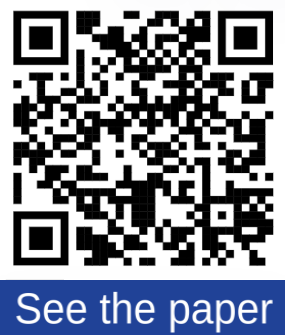
\includegraphics[height=5cm]{QRcode_arxiv2511.11548.png}%
}

% ====================
% Figure search path
% ====================
\graphicspath{{./figures/}}

% ====================
% Colours used in TikZ diagrams
% ====================
\definecolor{kdblue}{RGB}{0,112,192}

% ====================
% Body
% ====================
\begin{document}

\begin{frame}[t]

% ---- Banner figure at the top ----------------------------------------
\begin{figure}[h!]
  \centering
  
\includegraphics[width=0.8\textwidth, height=10cm, keepaspectratio=false]{periodic_universe.pdf}
\end{figure}

\begin{columns}[t]
\separatorcolumn

% ======================================================================
%  LEFT COLUMN
% ======================================================================
\begin{column}{\colwidth}
\vspace{-0.6cm}
  % ---- Block 1 : CPT-Symmetric Universe ----------------------------
  \begin{block}{Introduction: CPT-Symmetric Universe}
  Boyle \& Turok: the Big Bang acts as a \textbf{CPT mirror} \rightarrow can elegantly solve lots of problems in cosmology.
  \vspace{-0.5em}
    % \begin{itemize}
    %   \item Boyle \& Turok: the Big Bang acts as a \textbf{CPT mirror}
    %         joining our universe with an anti-universe on the other side
    %         [arXiv:2109.06204].
    %   \item \textbf{Direct evidence from CMB:} the ringing pattern in
    %         the CMB TT/TE power spectra implies a Neumann (reflecting)
    %         boundary condition at conformal time $\eta=0$:
    %         \[
    %           \dot\Phi\big|_{\eta=0}=0
    %           \;\Longleftrightarrow\;
    %           \text{Big Bang acts as a \textbf{temporal mirror}.}
    %         \]
    % \end{itemize}

    \begin{figure}[h!]
      \centering
      
\includegraphics[width=0.90\textwidth]{CPT_solve_problems.png}
    \end{figure}
  \end{block}

\vspace{-0.5em}
  % ---- Block 2 : Kähler–Dirac Fermions ----------------------------
  \begin{block}{Introduction: K\"{a}hler--Dirac Fermions}

    % \begin{columns}[c]
      % \begin{column}{0.60\colwidth}
      %   \textbf{Fermion doubling problem:} spinors have no natural
      %   $p$-form interpretation on a lattice $\Rightarrow$ extra
      %   doublers in the continuum limit; chiral theories become
      %   non-chiral (Nielsen--Ninomiya, 1981).

      %   \vspace{0.35em}
      %   \textbf{KD fermions} [K\"{a}hler, 1962] are $p$-forms ---
      %   they live naturally on any cell complex with \emph{no} doublers.
      %   This makes them ideal for lattice gauge theory.
      % \end{column}
    %   \begin{column}{0.36\colwidth}
    %     \begin{figure}[h!]
    %       \centering
    %       
\includegraphics[width=\textwidth]{lattice.png}
    %     \end{figure}
    %   \end{column}
    % \end{columns}

    \vspace{0em}
    \textbf{Differential-form formulation:}\\[0.2em]
    $\Phi = \sum_{p=0}^{4}\varphi_{\mu_1\cdots\mu_p}
    dx^{\mu_1}\!\wedge\cdots\wedge dx^{\mu_p}$\;
    is a polyform with $1+4+6+4+1=16$ complex components.
    \[
      S_{KD}=\langle\bar\Phi|(K-m)\Phi\rangle,
      \quad (K-m)\Phi=0,
      \quad K=d-d^\dagger, -K^2=\square.
    \]

    \textbf{Spinor formulation:} replacing $dx^\mu\to\gamma^\mu$
    assembles the 16 components into a $4\times4$ matrix $\Psi$:
    \[
      (i\gamma^\mu\partial_\mu - m)\Psi = 0,
      S_{KD} = \int d^4x\;\mathrm{Tr}
      \!\left[\bar\Psi(i\slashed\partial-m)\Psi\right],
       \bar\Psi\equiv\gamma^0\Psi^\dagger\gamma^0.
    \]
    Each column of $\Psi$ satisfies the ordinary Dirac equation.
    The symmetry group is $\mathrm{Spin}(3,1)_{\rm Lorentz}
    \times U(2,2)_{\rm internal}$.

  \end{block}


% ======================================================================
%  RIGHT COLUMN
% ======================================================================

\vspace{-0.5em}
  % ---- Block 3 : Wrong-sign, Two sheets, KD-Majorana, SM ----------
  \begin{block}{Negative-Norm States \& Two-Sheeted Spacetime}

    \textbf{Problem:} The extra $\gamma^0$ on the left of $\bar\Psi$ means half the columns have the wrong-sign Lagrangian. Diagonalising
    $\gamma^0=\Omega\Lambda\Omega^T$, with $\Lambda=\mathrm{diag}(+1,+1,-1,-1)$:
    \[
      S_{KD}=\int d^4x\;\mathrm{Tr}
      \!\left[\Lambda\,\Psi'{}^\dagger\gamma^0(i\slashed\partial-m)\Psi'\right],
      \quad \Psi'\equiv\Psi\Omega.
    \]
    Columns 3--4 of $\Psi'$ have the wrong sign
    $\Rightarrow$ \textbf{negative-norm states (ghosts)!}

    \vspace{0.3em}
    \textbf{Resolution [Donoghue \& Menezes, 2019]:}
    a wrong-sign action $=$ reversal of the causality arrow $=PT$ reversal.
    The two pairs of columns live on \textbf{two sheets of spacetime}, $PT$-mirrors of each other; both sheets have positive energy and norm.

\end{block}
\vspace{-0.5em}
\begin{block}{KD-Majorana condition \& SM Unification}
        \textbf{KD-Majorana condition:} to avoid coupling between two sheets and doubling of the particle content, impose
        \[
          \Psi^c\equiv(i\gamma^2)\Psi^*(i\gamma^2)=\Psi.
        \]
        This forces the four columns to take the form:
        \[
          \Psi'=\bigl(\psi_1,\;\psi_2,\;{-}\psi_2^c,\;\psi_1^c\bigr).
        \]
  \end{block}  
\end{column}

\separatorcolumn

\begin{column}{\colwidth}

    \begin{block}{}
    \begin{column}{0.6\colwidth}
        Every LH particle on the forward sheet is \emph{always} paired with a RH anti-particle on the backward sheet --- a manifestation of CPT symmetry. 
      \end{column}
      \begin{column}{0.38\colwidth}
      \vspace{-1cm}
        \begin{figure}[h!]
          \centering
          
\includegraphics[width=\textwidth]{KD_Majorana.png}
        \end{figure}
      \end{column}

    \vspace{0.3em}
    \textbf{SM fermion content in KD language:}
    one SM generation (including $\nu_R$) $= 4$ KD-Majorana fields
    $\Psi'_{A=0,1,2,3}$ (leptons $+$ three quark colours).
    All SM fermion kinetic \& Yukawa terms unify:
    \[
      \mathcal{L}_{\rm KD}=
        \mathrm{Tr}\!\left[\bar\Psi_A(i\slashed\partial)\Psi_A\right],
      \qquad
      \mathcal{L}_Y=
        \mathrm{Tr}\!\left[\mathcal{H}^T
        \widehat\Psi_{A,L}^{\prime\,i}\,\Psi_{A,R}^{\prime\,j}\,
        \mathcal{Y}_A^{ij}\right]+\text{h.c.}
    \]
    Gauging $SU(3)\!\subset\!SU(4)$ and
    $SU(2)\!\times\!U(1)\!\subset\!U(2,2)$ reproduces
    \emph{all} SM fermion gauge interactions.
    \textbf{$\nu_R$ is required by the geometry of the KD field.}

  \end{block}

  \vspace{-0.5em}

  % ---- Block 4 : Physical Implications ----------------------------
  \begin{block}{Physical Implications}

    \begin{columns}[t]

      % ---- Left sub-column : (1) CPT mirror + (2) BH mirror --------
      \begin{column}{0.48\colwidth}

        \textbf{(1) Theoretical Foundation of the CPT Mirror}
        \vspace{-0.4em}
        % The CPT-symmetric universe was motivated purely by CMB observations, with no theoretical explanation for why the
        % Big Bang \emph{must} be a CPT mirror.
        % The KD-Majorana condition provides the fundamental reason:
        \[
          \underbrace{\text{KD-Maj.}}_{\text{field theory}}
          \;\leftrightarrow\;
          \underbrace{\text{CPT mirror at Bang}}_{\text{cosmology}}
        \]
        % The Big Bang is precisely the junction where the two spacetime sheets meet.

        \vspace{0.6em}
        \textbf{(2) Black Mirror}
        {\small [arXiv:2412.09558]}

        \begin{itemize}\small
          \item The BH \emph{interior does not exist}
          \item The horizon mirrors our exterior to the ``other'' exterior (the anti-universe)
          \item Infalling particles \emph{annihilate} with anti-partners from the anti-universe at the horizon
          \item The KD-Majorana condition explains why every infalling particles are paired
        \end{itemize}

        \begin{figure}[h!]
          \centering
          
\includegraphics[width=0.80\textwidth]{annihilate_BHmirror.png}
        \end{figure}

      \end{column}

      % ---- Right sub-column : (3) Tenet ---------------------------
      \begin{column}{0.48\colwidth}

        \textbf{(3) Description of \textit{Tenet}?!}

        \begin{figure}[h!]
          \centering
          
\includegraphics[width=0.80\textwidth]{tenet_2.jpg}
        \end{figure}

        \vspace{0.2em}
        \textbf{\color{green!55!black}Same as CPT-sym. uni.:}
        \begin{enumerate}\small
          \item There is anti-universe with time goes backward
          \item The transition gates are \textbf{black holes}
        \end{enumerate}

        \vspace{0.3em}
        \textbf{\color{red!80!black}Difference from Tenet:}
        \begin{enumerate}\small
          \item You and anti-you \textbf{annihilate} at the transition gate (horizon)
          \item Viewed from our universe: you emerge from a \textbf{white hole} and find time reversed ---but you \emph{cannot change anything}, only re-experience the past
        \end{enumerate}

      \end{column}

    \end{columns}

  \end{block}
\vspace{-0.5em}
  \begin{block}{Future work}
   \begin{column}{\colwidth}
   \vspace{-1.7cm}
       \begin{enumerate}
           \item Construct KD Chiral gauge theory by considering two sheeted spacetime [Vaibhav, Latham (preparation)]
           \item String theory in 4D: consider KD fermions in superstring might form a ghost free theory without extra dimensions.
       \end{enumerate}
   \end{column}

  \end{block}
  
\end{column}

\separatorcolumn
\end{columns}
\end{frame}

\end{document}
